\subsection{Comparación de los sistemas al mismo tamaño}

La curva de los distintos experimentos ajustados sigue el mismo comportamiento 
para todos los sistemas, como se mostró en la Figura \ref{fig:ajustes-mapa},
esto es un efecto esperado debido a las definiciones de $\Xi$ y $\ell$, todas las
curvas exhiben una pendiente de $-1/2$ dada por la siguiente ecuación
\begin{equation}
    \log(\Xi) = \log(B) - \frac{1}{2}\log(\ell),
\end{equation}
donde el valor de $B$ puede obtenerse al eliminar C-rate de las ecuaciones 
\ref{eq:xi} y \ref{eq:ele} para obtener
\begin{equation}
    \log(\Xi) = \log(\frac{k^0 d}{D \sqrt{z}}) - \frac{1}{2}\log(\ell),
\end{equation}
donde se ve que la ordenada al origen contiene una composición de los parámetros
fundamentales considerados. 

\begin{figure*}[h!]
    \centering
    \begin{subfigure}{.575\textwidth}
        \centering
        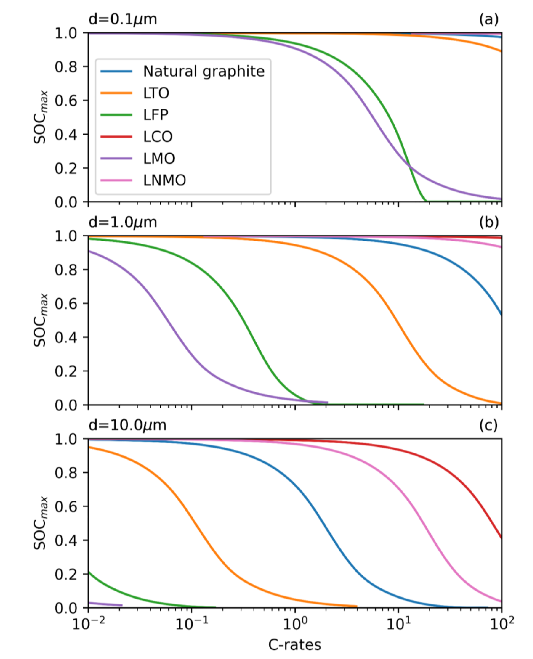
\includegraphics[height=.4\textheight]{FastCharging/un/resultados/comparacion/comparacion-curvas.png}
        \caption{Gráficos SOC$_{\max}$ \textit{versus} C-rate.}
        \label{fig:comparacion-curvas}
    \end{subfigure}
    \begin{subfigure}{.375\textwidth}
        \centering
        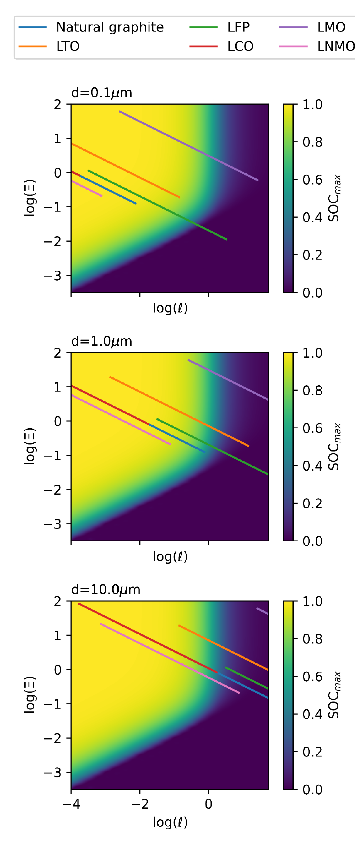
\includegraphics[height=.4\textheight]{FastCharging/un/resultados/comparacion/comparacion-mapa.png}
        \caption{Diagramas.}
        \label{fig:comparacion-mapa}
    \end{subfigure}
    \caption{Comparación de los sistemas considerados con distintos tamaños de 
    partícula entre 0.1 $\mu$m y 10.0 $\mu$m en el rango experimental usual para 
    valores de C-rates.}
    \label{fig:comparacion}
\end{figure*}

Si se quieren comparar los méritos de los distintos materiales, en términos de 
sus propiedades intrínsecas de transferencia de carga en la interfase 
electrodo/electrolito (k$^0$) y difusión de iones dentro de ellos ($D$), se 
debería comparar el comportamiento de las partículas para un mismo tamaño a 
distintas C-rate. Esto se presenta en la Figura \ref{fig:comparacion}. En 
particular, en la Figura \ref{fig:comparacion-curvas} se muestra el SOC$_{\max}$ 
en función de la C-rate, considerando un conjunto de tamaños de partículas y 
C-rates en un rango físicamente razonable. Para obtener estos resultados se 
utilizaron los valores de $D$ y $k^0$ ajustados en la sección \ref{s:ajustes}.

En el gráfico (i) de la Figura \ref{fig:comparacion-curvas} para 0.1 $\mu$m está
claro que los únicos materiales que muestran una pérdida de la capacidad para
C-rates altas son LFP y LMO, el resto retiene más del 80\% de la capacidad, 
incluso a 100 C. En el segundo gráfico (ii) de la Figura
\ref{fig:comparacion-curvas} para 1 $\mu$m, el LTO y el grafito amorfo tienen
una caída en el SOC por debajo del 50\% para 100 C, mientras que LCO y LNMO
están por encima del 80\%. Por último, el tamaño de partícula más grande que se 
considera, 10 $\mu$m (Figura \ref{fig:comparacion-curvas}, gráfico (iii)), 
todos los materiales presentan una retención de la capacidad por debajo del 80\%
a la C-rate más alta. En la Figure \ref{fig:comparacion-mapa} estos datos 
comportamientos están presentados en el diagrama construido con las simulaciones
galvanostáticas para dar una idea de las regiones en las que cada sistema se
encuentra. 

Cabe destacar que la secuencia de materiales dada en la Figura 
\ref{fig:comparacion} fue obtenida utilizando los valores de $k^0$ y $D$ 
ajustados con el modelo a los datos experimentales. Ajustar otros experimentos
podría alterar esta secuencia. Idealmente, las mediciones deberían estar 
realizadas sobre electrodos de una sola partícula.
